\documentclass[12pt]{article}
 \usepackage[margin=1in]{geometry} 
\usepackage{amsmath,amsthm,amssymb,amsfonts, enumitem, fancyhdr, color, comment, graphicx, environ}
\usepackage{booktabs}
\usepackage[colorinlistoftodos]{todonotes}
\usepackage{algorithm}
\usepackage{algpseudocode}
\usepackage{tikz}
\usepackage{subcaption}
\usepackage{float}
\usepackage{fancyhdr}
\usepackage{amsmath,amsthm,amssymb,amscd,epsfig,url}
\usepackage{fullpage}
\usepackage{times}
\usepackage{mathdots}
\newtheorem{theorem}{Theorem}[section]
\newtheorem{lemma}[theorem]{Lemma}
\newtheorem{proposition}[theorem]{Proposition}
\newtheorem{corollary}[theorem]{Corollary}
\newtheorem{conjecture}[theorem]{Conjecture}
\newtheorem{definition}[theorem]{Definition}
\newtheorem{example}[theorem]{Example}
\newtheorem{remark}[theorem]{Remark}
\usetikzlibrary{arrows.meta, automata, positioning}

\usepackage{listings}
\usepackage{xcolor}
\lstset{
  basicstyle=\ttfamily\small,
  backgroundcolor=\color{gray!10},
  frame=single,
  breaklines=true,
  keywordstyle=\color{blue},
  commentstyle=\color{gray},
  stringstyle=\color{red},
  showstringspaces=false,
  numbers=left,            
  numberstyle=\tiny\color{gray}, 
  numbersep=10pt 
}

%%%%%%%%%%%%%%%%%%%%%%%%%%%%%%%%%%%%%%%%%%%%%%%%%%%%%%%%%%%%%%%%%%%%%%%%
\pagestyle{fancy}
\fancyhf{}              % clear header + footer (important)
\fancyfoot[R]{\thepage} % page number bottom-right
\renewcommand{\headrulewidth}{0pt}

% make the title page (and other 'plain' pages) also show the number
\fancypagestyle{plain}{%
  \fancyhf{}
  \fancyfoot[R]{\thepage}
  \renewcommand{\headrulewidth}{0pt}
}


\setlength{\headheight}{14.5pt}
\newenvironment{problem}[2][Problem]{\begin{trivlist}
\item[\hskip \labelsep {\bfseries #1}\hskip \labelsep {\bfseries #2.}]}{\end{trivlist}}
\newenvironment{sol}
    {\emph{Solution:}
    }
    {
    \qed
    }
\specialcomment{com}{ \color{blue} \textbf{Comment:} }{\color{black}} %for instructor comments while grading
\NewEnviron{probscore}{\marginpar{ \color{blue} \tiny Problem Score: \BODY \color{black} }}

\newcounter{subproblem}
% \renewcommand{\thesubproblem}{\alph{subproblem}} % letters 
\renewcommand{\thesubproblem}{\arabic{subproblem}} % numbers
\newenvironment{subprob}[1][]{
  \refstepcounter{subproblem}
  \begin{trivlist}
  \item[\hskip \labelsep {\bfseries (\thesubproblem)}]
}{
  \end{trivlist}
}
\newenvironment{subsol}
    {\emph{Solution:}
    }
    {
    \qed
    }

% numbered within sections (optional)
% \newtheorem{theorem}{Theorem}[section]
% \newtheorem{lemma}[theorem]{Lemma} % shares theorem counter

%%%%%%%%%%%%%%%%%%%%%%%%%%%%%%%%%%%%%%%%%%%%%%%%%%%%%%%%%%%%%%%%%%%%%%%%%%%%%%%%%
\setlength {\marginparwidth }{2cm}
\newcommand{\nextline}{\\[0.2em]}

\newcommand{\R}{\mathbb{R}}
\newcommand{\N}{\mathbb{N}}
\newcommand{\Q}{\mathbb{Q}}
\newcommand{\Z}{\mathbf{Z}}
\newcommand{\st}{\text{ s.t }}
\newcommand{\tand}{\text{ and }}
\newcommand{\tor}{\text{ or }}
\newcommand{\bigO}[1]{\mathcal{O}\left(#1\right)}
\newcommand{\fP}{\mathbb{P}}
\newcommand{\E}{\mathbb{E}}


\usepackage{listings}
\usepackage{xcolor}
\lstset{
  basicstyle=\ttfamily\small,
  backgroundcolor=\color{gray!10},
  frame=single,
  breaklines=true,
  keywordstyle=\color{blue},
  commentstyle=\color{gray},
  stringstyle=\color{red},
  showstringspaces=false,
  numbers=left,            
  numberstyle=\tiny\color{gray}, 
  numbersep=10pt 
}


% titel en auteur van het document
\title{Problem Set \#5}
\author{Nicole Tian}
% \date{} % de datum van het document 

\begin{document}

\maketitle                  % maakt een kopje met titel, auteur 
\thispagestyle{empty}       % zet paginanummering uit voor deze 


\section*{Problem 0: Collaborators and Outside Sources}
Anthony Yoon, Michael Lee
\section*{Problem 1: Ford-Fulkerson (20 points)}
Graph:

    \begin{center}
    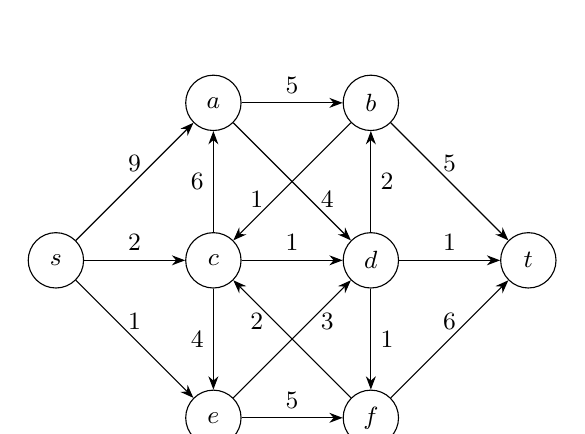
\begin{tikzpicture}[
      mycircle/.style={
         circle,
         draw=black,
         fill=white,
         fill opacity = 0.3,
         text opacity=1,
         inner sep=0pt,
         minimum size=20pt,
         font=\small},
      myarrow/.style={-Stealth},
      node distance=0.6cm and 1.2cm
      ]
      \node[mycircle]  at (-3, 0) (s) {$s$};
      \node[mycircle]  at (-1, 2) (a) {$a$};
      \node[mycircle]  at (1, 2) (b) {$b$};
      \node[mycircle]  at (-1, 0) (c) {$c$};
      \node[mycircle]  at (1, 0) (d) {$d$};
      \node[mycircle]  at (-1, -2) (e) {$e$};
      \node[mycircle]  at (1, -2) (f) {$f$};
      \node[mycircle]  at (3, 0) (t) {$t$};

    \foreach \i/\j/\txt/\p/\pp in {% start node/end node/text/position
      s.45/a.225/9/above/0.5,
      s.00/c.180/2/above/0.5,
      s.315/e.135/1/above/0.5,
      a.00/b.180/5/above/0.5,
      a.315/d.135/4/above/0.8,
      b.225/c.45/1/above/0.8,
      b.315/t.135/5/above/0.5,
      c.90/a.270/6/left/0.5,
      c.00/d.180/1/above/0.5,
      c.270/e.90/4/left/0.5,
      d.90/b.270/2/right/0.5,
      d.270/f.90/1/right/0.5,
      d.00/t.180/1/above/0.5,
      e.45/d.225/3/below/0.8,
      e.00/f.180/5/above/0.5,
      f.135/c.315/2/below/0.8,
      f.45/t.225/6/above/0.5
      }
       \draw [myarrow] (\i) -- node[font=\small,\p,pos=\pp] {\txt} (\j);


    \end{tikzpicture}
    \end{center}
\noindent Current flow:
    \begin{center}
    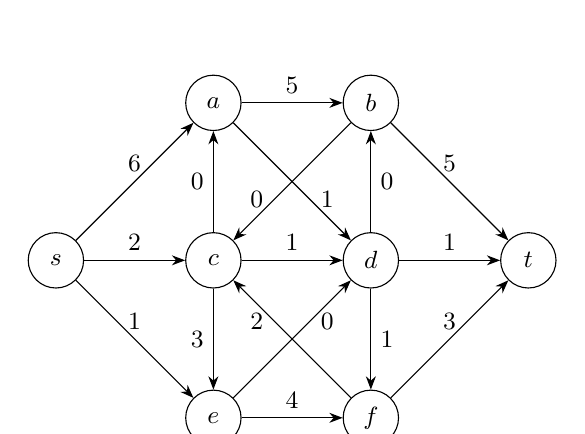
\begin{tikzpicture}[
      mycircle/.style={
         circle,
         draw=black,
         fill=white,
         fill opacity = 0.3,
         text opacity=1,
         inner sep=0pt,
         minimum size=20pt,
         font=\small},
      myarrow/.style={-Stealth},
      node distance=0.6cm and 1.2cm
      ]
      \node[mycircle]  at (-3, 0) (s) {$s$};
      \node[mycircle]  at (-1, 2) (a) {$a$};
      \node[mycircle]  at (1, 2) (b) {$b$};
      \node[mycircle]  at (-1, 0) (c) {$c$};
      \node[mycircle]  at (1, 0) (d) {$d$};
      \node[mycircle]  at (-1, -2) (e) {$e$};
      \node[mycircle]  at (1, -2) (f) {$f$};
      \node[mycircle]  at (3, 0) (t) {$t$};

    \foreach \i/\j/\txt/\p/\pp in {% start node/end node/text/position
      s.45/a.225/6/above/0.5,
      s.00/c.180/2/above/0.5,
      s.315/e.135/1/above/0.5,
      a.00/b.180/5/above/0.5,
      a.315/d.135/1/above/0.8,
      b.225/c.45/0/above/0.8,
      b.315/t.135/5/above/0.5,
      c.90/a.270/0/left/0.5,
      c.00/d.180/1/above/0.5,
      c.270/e.90/3/left/0.5,
      d.90/b.270/0/right/0.5,
      d.270/f.90/1/right/0.5,
      d.00/t.180/1/above/0.5,
      e.45/d.225/0/below/0.8,
      e.00/f.180/4/above/0.5,
      f.135/c.315/2/below/0.8,
      f.45/t.225/3/above/0.5
      }
       \draw [myarrow] (\i) -- node[font=\small,\p,pos=\pp] {\txt} (\j);


    \end{tikzpicture}
    \end{center}
Starting from the given flow, use the Ford-Fulkerson algorithm to find a maximum flow from $s$ to $t$ and find a minimum cut proving that this flow is a maximum flow. For each iteration (including the iteration where the algorithm terminates), show the residual graph and the flow path that you find from $s$ to $t$ (if such a path exists).\\
Note: If an edge in the residual graph has capacity $0$, showing this edge is optional (showing the edge or not showing the edge are both fine).

\begin{figure}[H]
  \centering
  \includegraphics[width=0.75\textwidth]{/Users/nyt/Theory of Algorithms/Problem_Set_5/Algorithms PSets.pdf}
  \caption{Example of a maximum flow of 11 from $s$ to $t$}
\end{figure}
There are no remaining paths on $s$ to $t$ on the residual graph. There is only one edge out of $s$ to $a$, and the only outward edges with nonzero capacity from vertices $a, b, d$ are to each other. Therefore, Ford-Fulkerson terminates sucessfully.


\section*{Problem 2: Tutoring Center (25 points)}
You are running a tutoring center where students meet with tutors at the center during various times of the week. You are trying to arrange weekly meetings between the students and the tutors and your constraints are as follows.
\begin{enumerate}
\item There are $n$ students $a_1,\ldots,a_n$, $n$ tutors $b_1,\ldots,b_n$, and $m$ time slots $t_1,\ldots,t_m$.
\item Each student $a_i$ wants to come in once a week to be tutored but can only come in for some subset $A_i$ of the time slots $t_1,\ldots,t_m$. Students do not have a preference among the tutors, they are satisfied as long as they are matched with a tutor.
\item Each tutor $b_j$ wants to come in once a week to tutor but can only come in for some subset $B_j$ of the time slots $t_1,\ldots,t_m$. Tutors do not have a preference among the students, they are satisfied as long as they are matched with a student.
\item For each time slot $t_k$, the center can only accomodate $c_k$ student/tutor meetings for some capacity $c_k$. This capacity may be different for different time slots due to other events at the center.
\end{enumerate}
You would like to schedule weekly meetings between the $n$ students and $n$ tutors, i.e., find triples $\{(a_i,b_{j_i},t_{k_i}): i \in [n]\}$ such that 
\begin{enumerate}
\item For all $i' \neq i$, $j_{i'} \neq j_{i}$ (each tutor tutors exactly once).
\item For all $i \in [n]$, $t_{k_i} \in A_i \cap B_{j_i}$ (both the student and the tutor are available for their time slot).
\item For all $k \in [m]$, $|\{i: k_i = k\}| \leq c_k$ (the capacity $c_k$ of each time slot $t_k$ is not exceeded).
\end{enumerate}
\begin{enumerate}
\item[(a)] Reudce problem down to a Max-Flow problem. We create a starting vertex $s$, $n$ vertices representing the students, $2$ sets of $m$ vertices representing the time slots ($2m$ total), $n$ vertices representing the tutors, and a ending vertex $t$. 

We create directed edges with capacity $1$ from $s$ to each of the students vertices. We create directed edges with capacity $1$ from each student to all time slots vertices they are available for. We create directed edges from each time slot vertex, $t_k$, to it's paired time slot vertex, $t_k'$ with capacity $c_k$. We create directed edges with capacity $1$ from each time slot to tutor vertices that are available during this time. Finally, we create directed edges with capacity $1$ from each tutor vertex to $t$.

We use Ford-Fulkerson to then solve the resulting max-flow problem and read off the schedule from the integral flow to find pairings of students and tutors.

\item[(b)] 
\textbf{If there exists a schedule $\{(a_i, b_{j_i}, t_{k_i}) | i \in [n]\}$ which matches $n$ students with $n$ tutors}, then there exists a flow of $n$ from $s$ to $t$. We can direct a flow of $1$ from $s$ to each student $a_i \in [n]$. Then we can direct flow from each student to time slot $t_{k_i}$, to it's duplicate $t_{k_i}'$, another flow to $b_{j_i}$ and then finally to $t$. 
This is possible by definition of the schedule. A flow of $1$ from each $a_i$ to time slot $t_{k_i}$ is always possible by construction. Let $p_{k_i}$ represent the number of student/teacher pairs using time slot $t_{k_i}$. By property of the schedule, $p_{k_i} \leq c_k$, therefore the flow from time slot $t_{k_i}$, to it's duplicate $t_{k_i}'$ of $p_{k_i}$ is possible. The flow from $t_{k_i}'$ to $b_{j_i}$ is possible since no teacher is scheduled more than once. Finally, a flow of $1$ from each $b_{j_i}$ to $t$ is always possible by construction. Since there are $n$ pairs, this is a flow of $n$.

\textbf{If there exists a flow of value $n$ from $s$ to $t$}, we can find a schedule which matches $n$ students to $n$ teachers by following the flow from each student $a_i$ to a time slot $t_{k_i}$ and then to a teacher $b_{j_i}$. This satisifies all the requirements of the schedule.
\begin{enumerate}
\item[] All tutors are used once. Otherwise, the number of tutors used is less than $n$. And since $f_{out}(b_{j_i}) = 1$, the max flow is less than $n$. Therefore each teacher is paired with only $1$ student.

\item[] Both student and tutor are available for their time slot. By construction, there exists only edges between $a_i$ and $t_{k_i}$ if $a_i$ is available during $t_{k_i}$ and there exists only edges between $t_{k_i}'$ and $b_{j_i}$ if $b_{j_i}$ is available during $t_{k_i}'$. Therefore, for there to be a flow connecting $a_i$ to a time slot $t_{k_i}$ and then to a teacher $b_{j_i}$, that means both $a_i$ and $b_{j_i}$ are available during $t_{k_i}$.

\item[] Capacity is not exceeded. For each $t_{k_i}$, $f_{out}(t_{k_i}), f_{in}(t_{k_i})\leq c_k$. Therefore the number of students that are occuping time slot $t_{k_i}$ is less than or equal to $c_k$.
\end{enumerate}

\item[(c)] Creating the graph $G$ requires going through all students, connecting it with available time slots and then connecting time slots with available tutors which is $O(nm)$. (Creating all other edges takes linear time.)

Running Ford-Fulkerson is $O((nm) \times n) \Rightarrow O(\max(n^2m))$

Total time complexity is $O(\max(n^2m))$
\end{enumerate}

\section*{Problem 3: Carpooling (Rephrasing of problem 27 in Chapter 7 of Kleinberg-Tardos, 30 points, 5 extra credit points available)}
A group of $k$ people $p_1,\ldots,p_k$ are carpooling to work for $n$ days and they need to choose drivers for each day. However, only a subset of the people go to work each day. Also, they would like to divide up the driving duties fairly. In particular, no person should drive more than the expected number of times they would drive if the driver was chosen randomly each day (rounded up).
\begin{example}
Let's say there are 3 people $p_1,p_2,p_3$ carpooling for 4 days and the people carpooling on each day are as follows:
\begin{enumerate}
\item On day $1$, all $3$ people are carpooling.
\item On day $2$, $p_1$ and $p_3$ are carpooling.
\item On day $3$, $p_2$ and $p_3$, are carpooling.
\item On day $4$, $p_2$ and $p_3$ are carpooling again.
\end{enumerate}
In this case, if the driver was chosen randomly each day, the expected number of times $p_1$ drives is $\frac{1}{3} + \frac{1}{2} = \frac{5}{6}$. The expected number of times $p_2$ drives is $\frac{1}{3} + 2\cdot\frac{1}{2} = \frac{4}{3}$. The expected number of times $p_3$ drives is $\frac{1}{3} + 3\cdot\frac{1}{2} = \frac{11}{6}$. Thus, we can have $p_1$ drive at most $1$ time and we can have $p_2$ and $p_3$ drive at most $2$ times. One way to do this is to have $p_1$ drive on day $2$, have $p_2$ drive on day $3$, and have $p_3$ drive on days $1$ and $4$
\end{example}
We can state this problem more precisely as follows. We are given subsets the subsets of people $\{S_j\}$ who are carpooling each day and we want to choose drivers $\{p_{i_j}\}$ such that 
\begin{enumerate}
\item $\forall j \in [n] (i_j \in S_j)$ (the driver for each day is one of the people carpooling for that day)
\item $\forall i \in [k]\left(|\{j: i_j = i\}| \leq \lceil\sum_{j \in [n]:i \in S_j}{\frac{1}{|S_j|}}\rceil\right)$ (no person drives more than the expected number of times they should drive rounded up)
\end{enumerate}
\begin{enumerate}
\item[(a)]

\textbf{Algorithm}

Reudce problem down to a Max-Flow problem. We create a graph $G$ with vertex $s$ representing the source, vertices $d_1,\dots,d_n$ representing the days, vertices
$p_1,\dots,p_k$ representing the people, and vertex $t$ representing the end. We assign capacities as follows:
\begin{enumerate}
  \item $s\to d_j \text{ has capacity }1$
  \item $d_j\to p_i \text{ has capacity }1 \text{ if } p_i\in S_j$
  \item $p_i\to t \text{ has capacity }c_i$
\end{enumerate}

\[c_i = \lceil\sum_{j \in [n]:i \in S_j}{\frac{1}{|S_j|}}\rceil\]

We use Ford-Fulkerson to solve the resulting max-flow problem. If the max flow is less than $n$, a schedule that satisifies the requirements does not exist. This is because each $n$ day gets sent a flow of $1$ from $s$. In order to get a max flow of $n$, every day needs to send it's $1$ unit of flow forward to a driver. 

If a valid schedule exists, to find it, we look at each day. For each day $j$, look for the edge $d_j \rightarrow p_i$ with flow $1$ and set $p_{j_i} = p_i$

\textbf{Existance of Schedule:} Assume $|S_j|\ge 1$ for every day $j\in\{1,\dots,n\}$.  
Let
\[
c_i \;=\;\left\lceil \sum_{j:\, p_i\in S_j}\frac{1}{|S_j|}\right\rceil .
\]
Then there always exists a choice of drivers $p_{i_1},\dots,p_{i_n}$ such that $p_{i_j}\in S_j$ for each day $j$, and each person $p_i$ drives at most $c_i$ times.

\begin{proof}
Build the graph $G$ as stated above: source $s$, day-nodes $d_1,\dots,d_n$, person-nodes
$p_1,\dots,p_k$, end $t$, with the following capacities:
\begin{enumerate}
  \item $s\to d_j \text{ has capacity }1$
  \item $d_j\to p_i \text{ has capacity }1 \text{ if } p_i\in S_j$
  \item $p_i\to t \text{ has capacity }c_i$
\end{enumerate}

The total capacity out of $s$ is $n$, so any $s$-$t$ flow has value at most $n$. Therefore to prove that every $s$-$t$ cut has capacity of exactly $n$, it is sufficent to prove that every $s$-$t$ cut has capacity of at least $n$. 

Let $(L,R)$ be any cut with $s\in L$ and $t\in R$. Let
\[
D_L = \{j : d_j\in L\} \tand P_L=\{i : p_i\in L\}.
\]
We define $D_R$ and $P_R$ similarly.

We transform the cut st. there exists no edges crossing from $D_L \rightarrow P_R$ without changing the capacity of the cut. If there is a day node $d_j\in D_L$ and a person node $p_i\in P_R$ with an edge $d_j\to p_i$, then that edge contributes $1$ to the cut capacity. We can move $d_j$ to $R$. This removes all crossing edges out of $d_j$ (each of capacity $1$) and adds
only the single edge $s\to d_j$ of capacity $1$, so the cut capacity does not increase.
Repeating this for all such pairs, we may assume that if $d_j\in L$, then $S_j \subseteq P_L$. 

No edges $d_j\to p_i$ cross the cut, so the only edges from $L$ to $R$ are edges $s\to d_j$ with $d_j\in R$, contributing $n-|D_L|$, and edges $p_i\to t$ with $p_i\in L$, contributing $\sum_{i\in P_L} c_i$.

Hence the cut capacity is
\[
\mathrm{cap}(L,R) = (n-|D_L|) + \sum_{i\in P_L} c_i .
\]
So it suffices to show $\sum_{i\in P} c_i \ge |D_L|$.

Since there are no crossing edges, $S_j\subseteq P_L$ for every $j\in D_L$. Therefore
\[
|D_L|
= \sum_{j\in D_L} 1
= \sum_{j\in D_L}\sum_{p_i\in S_j}\frac{1}{|S_j|}
= \sum_{i\in P}\;\sum_{j\in D_L | p_i\in S_j}\frac{1}{|S_j|}.
\]
For each fixed $i\in P$,
\[
\sum_{j\in D_L | p_i\in S_j}\frac{1}{|S_j|}
\le
\left\lceil \sum_{j\in D_L | p_i\in S_j}\frac{1}{|S_j|}\right\rceil
= c_i .
\]
\[\Rightarrow \sum_{i\in P} c_i \ge |D_L|\]

Therefore every cut has capacity at least $n$, and by containment, the maximum flow value is exactly $n$.

Finally, since all capacities are integers, there exists an integral max flow. Reading off the
unique edge from each $d_j\to p_i$ with flow $1$ assigns a driver $p_i\in S_j$ to each day $j$, and the
capacity $c_i$ on $p_i\to t$ ensures person $p_i$ is chosen at most $c_i$ times. This is a
valid schedule.
\end{proof}

\item[(c)] Creating the graph $G$ is $O(nk)$. Ford-Fulkerson is $O(nk * n)$. Therefore the total time complexity is $O(n^2k)$
\item[(d)] \textbf{Example}

Let there be $n=3$ days and $k=2$ people, $p_1,p_2$.  Define the sets of people who go to work each day:
\begin{enumerate}
  \item $S_1=\{p_1,p_2\}$
  \item $S_2=\{p_1\}$
  \item $S_3=\{p_2\}$
\end{enumerate}

Then each person goes to work on exactly $2$ of the $3$ days, and each day has either $1$ or $2$ people. Therefore the expected value of drives per person is $\frac{1}{1} + \frac{1}{2}$. If we rounded down, we get a value of $1$.

But there are $3$ days and the rounding-down
bounds allow at most $1+1=2$ total drives. Hence no valid schedule can exist under rounding down.
\end{enumerate}


\section*{Problem 4: Evacuating a Graph (25 points)}
Let's say that we are trying to evacuate people from a graph. More precisely, we have the following setup:
\begin{enumerate}
\item We have a connected undirected graph $G$ with $n$ vertices and $m$ edges.
\item Initially, there are $k$ people at some set $S = \{s_1,\ldots,s_k\} \subseteq V(G)$ of the vertices of the graph.
\item There is a set $T = \{t_1,\ldots,t_r\} \subseteq V(G)$ of exit vertices such that if a person is currently at a vertex $t_i \in T$ then they can immediately exit the graph during the next time step.
\item During each time step, a person can either exit the graph if they are at a vertex in $T$ or move from their current vertex to an adjacent vertex if they are at some other vertex. However, each vertex can only have one person at a time. In particular, while it is okay for a person to move to an occupied vertex if the person there is moving to a different vertex or escaping the graph, we can never have two or more people move to the same vertex and we cannot have a person move to an occupied vertex if the person there is staying put for this time step. 
\end{enumerate}
\begin{enumerate}
\item[(a)] \textbf{Algorithm}

Fix an integer $l \ge 0$. We build a directed graph $G_l$
and check whether all $k$ people can evacuate within $l$ time steps by computing a max flow. If the max flow value is $k$, then all $k$ people can evacuate within $l$ steps.

Then we binary search over all possible $l$ between $0 \tand n^2$ to find minimum $l$ s.t. all $k$ people can evacuate.

\noindent\textbf{Vertices:}
For each vertex $v\in V(G)$ and each time $i \in\{0,1,\dots, l\}$ create three vertices
$v_{\mathrm{in}}^{(i)}, v_{\mathrm{out}}^{(i)} \tand v_{\mathrm{in}}^{(i+1)}$. Create a source vertex $s$ and end vertex $t$.

\noindent\textbf{Edges and capacities:}
\begin{enumerate}
\item For every $v\in V(G)$ and every $i\in\{0,1,\dots,l\}$ add $v_{\mathrm{in}}^{(i)} \to v_{\mathrm{out}}^{(i)}$ with capacity 1
\item For every $v\in V(G)$ and every $i\in\{0,1,\dots,l-1\}$ add $v_{\mathrm{out}}^{(i)} \to v_{\mathrm{in}}^{(i+1)} \text{with capacity }1$

\item For each starting location $s_j\in S=\{s_1,\dots,s_k\}$ add $s \to (s_j)_{\mathrm{in}}^{(0)} \text{with capacity } 1$

\item For each time $i\in\{0,1,\dots,l-1\}$ and each undirected edge $\{u,v\}\in E(G)$ add $ u_{\mathrm{out}}^{(i)} \to v_{\mathrm{in}}^{(i+1)} \text{cap }1, \tand
v_{\mathrm{out}}^{(i)} \to u_{\mathrm{in}}^{(i+1)} \quad \text{cap }1$

\item For each exit vertex $x\in T$ and each time $i\in\{0,1,\dots,l-1\}$ add $ x_{\mathrm{out}}^{(i)} \to t \text{ with capacity } 1$
\end{enumerate}

\noindent\textbf{Finding evacuation routes:}
Once we find our minimum $l$ with max flow of $k$, we can decompose the flow into $k$ paths from $s$ to $t$. Each path specifies, for each time $i \in \{0, 1, \dots, l\}$, which vertex the corresponding person occupies, giving evacuation routes.

\item[(b)] If there is a valid evacuation schedule of length $l$, then for each person we send
one unit of flow along the corresponding time-respecting path through $G_l$. The edges exist exactly for legal moves/waits/exits, and the capacity $1$ vertex-splitting edges enforce that no vertex contains more than one person at the same time. Hence we get a feasible flow of value $k$.

Conversely, if there is an integral flow of value $k$, we can decomposing it into $k$ paths containing some $s_i \in S$ and some $x \in T$, yielding $k$ evacuation routes. The capacity $1$ constraint through each $v^{(i)}$ guarantees that at most one path uses vertex
$v$ at time $i$, and moves/waits/exits are legal by construction.

Binary search returns the minimum $l$ because if evacuation is possible in $l$ steps it is also possible in $l+1$ steps (invariant).

\item[(c)]
\textbf{For a fixed $l$}, the graph has $nl$ vertices and $O(nl) + O(n) + O(lm) + O(nl) \Rightarrow O(l(n+m))$ edges

Therfore creating $G_l$ is $O(l(n+m))$ and running Ford-Fulkerson is $O((ln(n+m)))$

$\Rightarrow O(ln(n+m))$


Binary searching over $l \in\{0,1,\dots,n^2\}$ adds a factor of $O(\log n^2)$ and in the worst case, $l = n^2$. The total runtime is $O(\log n^2 * [n^3(n+m)])$.
\end{enumerate}

\end{document}
